\chapter{التوازن الكيميائي: خارج التفاعل وثابت التوازن}\label{ch:g12:equilibrium}

قارورة ماء فوّار مغلقة تحفظ فورانها شهورًا؛ فإذا فُتحت
فقدته في عصر واحد. ولا خلل في أي من الحالتين. ففي
القارورة المغلقة، يغادر ثنائي أكسيد الكربون الماء ويعود إليه بالسرعة
نفسها، فيبقى التركيب على حاله؛ فإذا فُتحت السدادة، لم يعد الغاز الذي
يغادر يرجع. وكثير من التفاعلات تسلك هذا السلوك: فهي تتوقف
قبل أن يُستهلك أي \omterm{def:g7:chemical-reactions:reactant}{متفاعل}، عند توازن بين تفاعلين
متعاكسين. وهذا الفصل يصف ذلك التوازن بعدد واحد.

\begin{recall}
\omterm{def:g10:reaction-progress-table:extent}{تقدم التفاعل} $x$، وقيمته القصوى $x_{\max}$، والتفاعلات
التامة التي تبلغها (\cref{ch:g10:reaction-progress-table}). السرعات
والعوامل الحركية (\cref{ch:g12:reaction-rates})؛ \omterm{def:g12:catalysis:catalyst}{والحفّاز} لا يغيّر
\omterm{def:g10:reaction-progress-table:system}{الحالة النهائية} (\cref{ch:g12:catalysis}).
\end{recall}

\begin{omfigure}
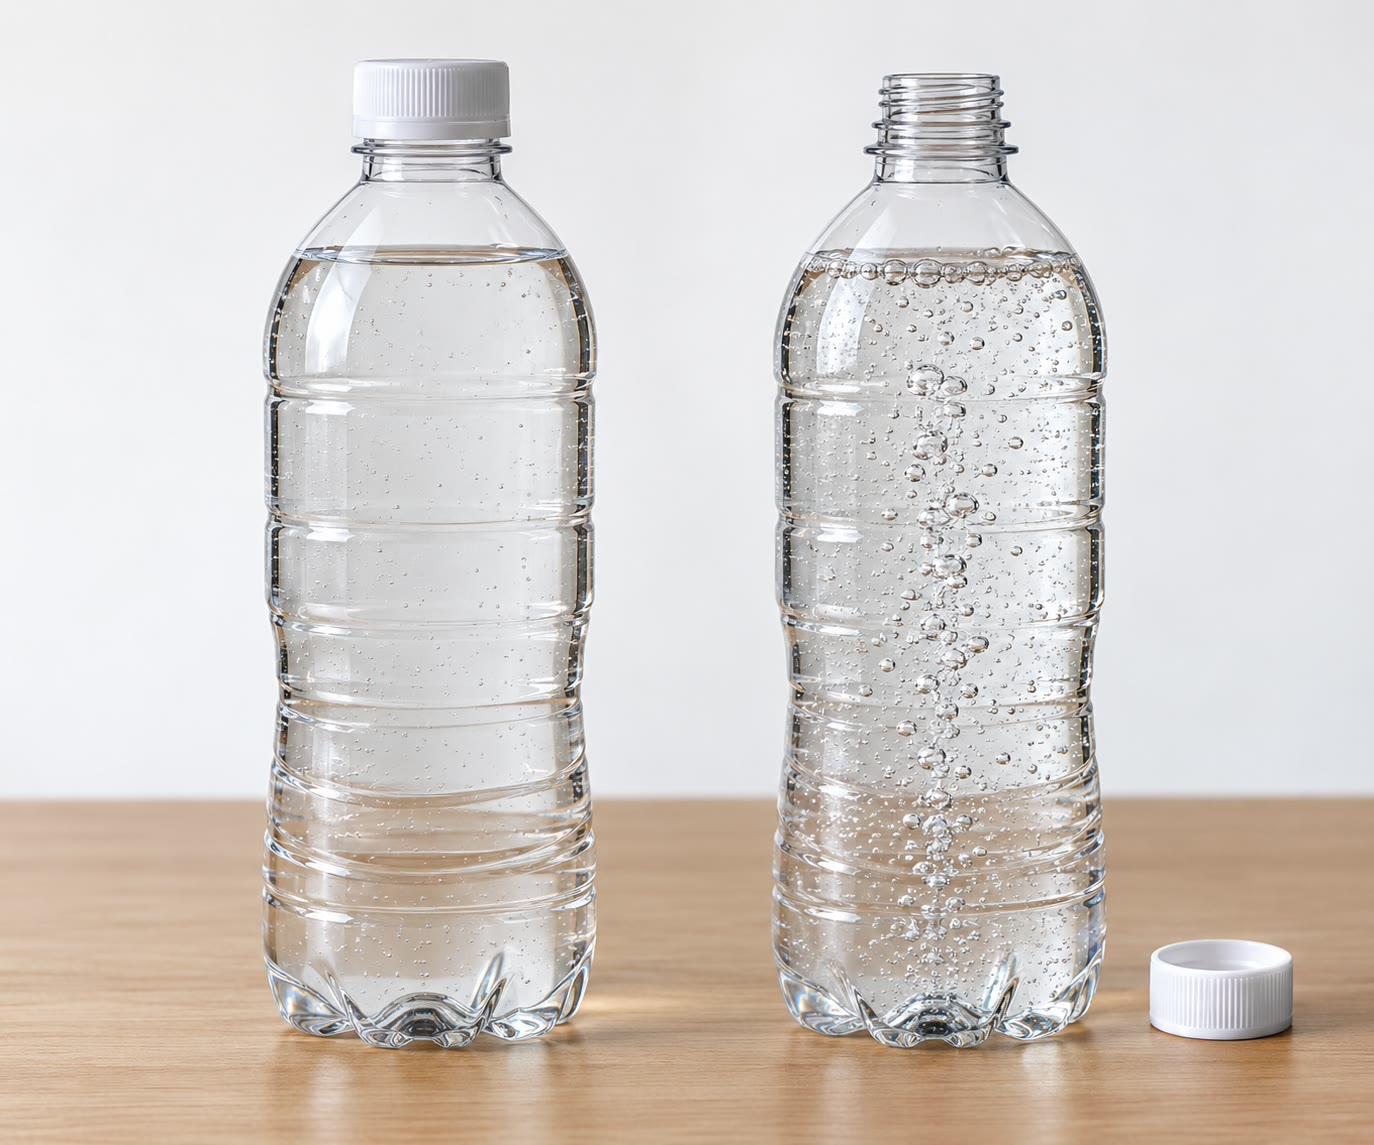
\includegraphics[width=0.45\linewidth,height=5cm,keepaspectratio]{images/book1/ai/g12-fizzy-bottles.jpg}

{\small مغلقةً، يحفظ الماء غازه؛ ومفتوحةً، يفلت الغاز ولا
يعود.}
\end{omfigure}

\section{تفاعلات غير تامة}

\begin{definition}[التفاعل غير التام، نسبة التقدم النهائي]\label{def:g12:equilibrium:non-total}
يكون التفاعل \emph{تفاعلًا غير تام}\index{تفاعل غير تام} إذا
توقف عند تقدم نهائي $x_f$ أصغر من تقدمه الأقصى $x_{\max}$،
\omterm{def:g7:chemical-reactions:reactant}{والمتفاعلات} كلها ما زالت موجودة. و\emph{نسبة التقدم
النهائي}\index{نسبة التقدم النهائي} له هي
\[
  \tau = \frac{x_f}{x_{\max}}, \qquad 0 < \tau < 1
\]
($\tau = 1$ \omterm{def:g10:reaction-progress-table:limiting}{للتفاعل التام}).
\end{definition}

\begin{example}[إستر يتوقف في منتصف الطريق]\label{ex:g12:equilibrium:berthelot}
% ledger: ester:berthelot
إذا سُخّن \qty{1}{mol} من حمض الإيثانويك مع \qty{1}{mol} من الإيثانول، تكوّن
إيثانوات الإيثيل والماء،
\ce{CH3COOH + C2H5OH <=> CH3COOC2H5 + H2O}. ويتوقف التفاعل حين يكون نحو
ثلثي الحمض قد تفاعلا: $x_f = \qty{0.67}{mol}$ مقابل
$x_{\max} = \qty{1}{mol}$، إذن $\tau \approx 0.67$. وانطلاقًا من
\qty{1}{mol} من \omterm{def:g11:functional-groups:carboxylic-acid}{الإستر} و\qty{1}{mol} من الماء، يتوقف التفاعل العكسي
أيضًا، بعد حلمأة نحو ثلث \omterm{def:g11:functional-groups:carboxylic-acid}{الإستر}: فنصل إلى \omterm{def:g6:pure-substances-and-mixtures:mixture}{الخليط}
النهائي نفسه.
\end{example}

\begin{history}[برتلو وبيان دو سان-جيل، 1862]
% ledger: ester:berthelot
سخّن الكيميائيان مارسلان برتلو وليون بيان دو سان-جيل
مخاليط من حمض الإيثانويك والإيثانول، ومن إيثانوات الإيثيل والماء،
مددًا طويلة، ثم حلّلاها. فمن كميتين متساويتين من الحمض
\omterm{def:g11:functional-groups:alcohol}{والكحول}، كان التفاعل يتوقف دائمًا عند نحو الثلثين؛ ومن \omterm{def:g11:functional-groups:carboxylic-acid}{الإستر}
والماء، عند حلمأة الثلث؛ ولاحظا أن كمية
\omterm{def:g11:functional-groups:carboxylic-acid}{الإستر} المتكوّنة في كل لحظة تتوقف على جداء كميتي
المتفاعلين. وكان عملهما من أولى الدراسات الكمية
لتوازن كيميائي.
\end{history}

\section{حالة التوازن}

\begin{definition}[حالة التوازن]\label{def:g12:equilibrium:equilibrium-state}
تكون المجموعة في \emph{حالة توازن}\index{حالة توازن} حين
لا يعود تركيبها يتغير مع أن التفاعلين المباشر
والعكسي ما زالا يجريان، بالسرعة نفسها. والتفاعل الذي
يمكن أن يبلغ حالة كهذه يُكتب بالسهم المزدوج $\rightleftharpoons$.
\end{definition}

\begin{omfigure}
\begin{tikzpicture}
\begin{axis}[width=0.8\linewidth, height=6cm, xmin=0, xmax=200, ymin=0,
    ymax=1.05, xlabel={\babelsublr{$t$ (\si{h})}}, ylabel={\foreignlanguage{arabic}{كمية الإستر \babelsublr{(\si{mol})}}},
    axis lines*=left, ymajorgrids, grid style={gray!20},
    tick label style={font=\small}, label style={font=\small},
    legend style={font=\small, at={(0.98,0.98)}, anchor=north east,
    draw=none, fill=white}, legend cell align=left]
  % ledger: ester:berthelot (K = 4; kinetics synthetic)
  \addplot[very thick, omDef] table[x=t, y=fromAcid] {figdata/out/grade-12-equilibrium.dat};
  \addplot[very thick, omProp] table[x=t, y=fromEster] {figdata/out/grade-12-equilibrium.dat};
  \addplot[dashed, black!60] coordinates {(0,0.6667) (200,0.6667)};
  \legend{{\foreignlanguage{arabic}{من \babelsublr{1} \babelsublr{mol} حمض + \babelsublr{1} \babelsublr{mol} كحول}}, {\foreignlanguage{arabic}{من \babelsublr{1} \babelsublr{mol} إستر + \babelsublr{1} \babelsublr{mol} ماء}}}
  \node[font=\small, anchor=north east] at (axis cs:195,0.65) {\foreignlanguage{arabic}{التوازن: $\tfrac{2}{3}$ \babelsublr{mol}}};
\end{axis}
\end{tikzpicture}

{\small تبلغ الأسترة (بالأزرق) وحلمأة \omterm{def:g11:functional-groups:carboxylic-acid}{الإستر}
(بالبرتقالي) تركيب التوازن نفسه، من جهتين متقابلتين.
(السلّم الزمني نموذجي؛ أما القيمة النهائية فمقيسة.)}
\end{omfigure}

\section{خارج التفاعل}

\begin{notation}[التركيز المرجعي]\label{not:g12:equilibrium:c-standard}
$c^\circ = \qty{1}{mol/L}$ هو التركيز المرجعي. وقسمة
تركيز على $c^\circ$ تعطي عددًا بلا وحدة له
القيمة نفسها: $[\ce{A}]/c^\circ$.
\end{notation}

\begin{definition}[خارج التفاعل]\label{def:g12:equilibrium:quotient}
لتفاعل في \omterm{def:g2:mixing-and-dissolving:dissolve}{محلول} $a\,\ce{A} + b\,\ce{B} \rightleftharpoons c\,\ce{C} + d\,\ce{D}$، يكون \emph{خارج
التفاعل}\index{خارج التفاعل} في حالة معيّنة للمجموعة
\[
  Q = \frac{\left([\ce{C}]/c^\circ\right)^c \left([\ce{D}]/c^\circ\right)^d}
           {\left([\ce{A}]/c^\circ\right)^a \left([\ce{B}]/c^\circ\right)^b} .
\]
لا تظهر الأجسام الصلبة، ولا \omterm{def:g6:solutions-and-solubility:solute}{المذيب} (الماء في \omterm{def:g6:solutions-and-solubility:solute}{محلول مائي})، في
$Q$.
\end{definition}


\begin{example}[كتابة خوارج التفاعل]\label{ex:g12:equilibrium:quotients}
للتفاعل \ce{CH3COOH + H2O <=> CH3COO- + H3O+} في الماء (يُقدَّم \omterm{def:g9:ions:ion}{الأيون} \ce{H3O+}
في الفصل التالي)، الماء هو \omterm{def:g6:solutions-and-solubility:solute}{المذيب}:
$Q = \dfrac{[\ce{CH3COO-}]\,[\ce{H3O+}]}{[\ce{CH3COOH}]\,c^\circ}$. ولذوبان
جسم صلب، \ce{AgCl(s) <=> Ag+ + Cl-}، يُستبعد الصلب:
$Q = [\ce{Ag+}][\ce{Cl-}]/(c^\circ)^2$. وللأسترة، حيث الأنواع الأربعة
كلها في \omterm{def:g6:pure-substances-and-mixtures:mixture}{الخليط} السائل نفسه ذي الحجم $V$، تُحذف الأحجام
فيكون $Q = \dfrac{n_{\text{إستر}}\, n_{\text{ماء}}}{n_{\text{حمض}}\, n_{\text{كحول}}}$.
\end{example}

\section{ثابت التوازن}

\begin{definition}[ثابت التوازن]\label{def:g12:equilibrium:constant}
قيمة $Q_{eq}$ \omterm{def:g12:equilibrium:quotient}{لخارج التفاعل} في \omterm{def:g12:equilibrium:equilibrium-state}{حالة التوازن} هي
\emph{ثابت التوازن}\index{ثابت التوازن} $K$ لهذا
التفاعل. ولا وحدة له.
\end{definition}

\begin{proposition}[لا يتوقف $K$ إلا على درجة الحرارة]\label{prop:g12:equilibrium:constant}
لتفاعل معيّن، $Q_{eq} = K$ في كل \omterm{def:g12:equilibrium:equilibrium-state}{حالة توازن} عند درجة حرارة
معيّنة، مهما كانت الكميات الابتدائية.
\end{proposition}

\begin{proof}
نقبله؛ ويُستنتج في مجلد السنة الثانية. ونتحقق منه على
الأسترة: فالتجربتان في الشكل، المبدوءتان من جهتين متقابلتين،
تعطيان $Q_{eq}$ نفسه.
\end{proof}

\begin{example}[ثابت $K$ للأسترة]\label{ex:g12:equilibrium:k-ester}
% ledger: ester:berthelot
انطلاقًا من \qty{1}{mol} من الحمض و\qty{1}{mol} من \omterm{def:g11:functional-groups:alcohol}{الكحول}، يحوي التوازن
$\frac{2}{3}$ mol من \omterm{def:g11:functional-groups:carboxylic-acid}{الإستر} ومثلها من الماء و$\frac{1}{3}$ mol من
الحمض ومثلها من \omterm{def:g11:functional-groups:alcohol}{الكحول}:
\[
  K = \frac{(2/3)\times(2/3)}{(1/3)\times(1/3)} = 4 .
\]
\end{example}

\begin{method}[الحالة النهائية لتفاعل غير تام]\label{met:g12:equilibrium:final}
\begin{enumerate}
  \item املأ \omterm{def:g10:reaction-progress-table:extent}{جدول التقدم} بالتقدم النهائي المجهول $x_f$.
  \item اكتب $Q_{eq}$ بدلالة $x_f$ وساوِ بينه وبين $K$.
  \item احسب $x_f$ (وكثيرًا ما تكون المعادلة من الدرجة الثانية)، محتفظًا بالجذر
        الواقع بين 0 و$x_{\max}$.
  \item استنتج الكميات النهائية و$\tau = x_f/x_{\max}$.
\end{enumerate}
\end{method}

\begin{example}[فائض من الكحول]\label{ex:g12:equilibrium:excess}
انطلاقًا من \qty{1}{mol} من الحمض و\qty{2}{mol} من \omterm{def:g11:functional-groups:alcohol}{الكحول}:
$\dfrac{x^2}{(1-x)(2-x)} = 4$، أي $3x^2 - 12x + 8 = 0$، وجذرها
الواقع بين 0 و1 هو $x_f = \qty{0.845}{mol}$. فمضاعفة \omterm{def:g11:functional-groups:alcohol}{الكحول} ترفع
\omterm{def:g10:synthesis-yield:yield}{المردود}، محسوبًا على الحمض، من \qty{67}{\percent} إلى
\qty{85}{\percent}.
\end{example}

\section{التنبؤ بالتطور وإزاحته}

\begin{proposition}[اتجاه التطور]\label{prop:g12:equilibrium:direction}
إذا كان $Q < K$، تطورت المجموعة في الاتجاه المباشر (تزداد
\omterm{def:g7:chemical-reactions:reactant}{النواتج}) حتى يصير $Q = K$؛ وإذا كان $Q > K$، تطورت في الاتجاه العكسي؛
وإذا كان $Q = K$، فهي في توازن ولا تتغير.
\end{proposition}

\begin{proof}
نقبله: \omterm{def:g12:equilibrium:quotient}{فخارج التفاعل} $Q$ يزداد حين يتقدم التفاعل المباشر (\omterm{def:g7:chemical-reactions:reactant}{فالنواتج} في
البسط تزداد، \omterm{def:g7:chemical-reactions:reactant}{والمتفاعلات} في المقام تنقص)، والمجموعة
تتجه نحو الحالة التي يكون فيها $Q = K$.
\end{proof}

\begin{omfigure}
\begin{tikzpicture}[font=\small]
  \draw[->, thick] (0,0) -- (10,0) node[right] {$Q$};
  \draw[thick] (0,-0.12) -- (0,0.12) node[above] {0};
  \draw[very thick, omThm] (5,-0.25) -- (5,0.25) node[above] {$K$};
  \draw[->, very thick, omDef] (1.2,0.55) -- (4.4,0.55);
  \node[omDef, align=center] at (2.8,1.15) {\foreignlanguage{arabic}{$Q < K$: مباشر}};
  \draw[->, very thick, omProp] (8.8,0.55) -- (5.6,0.55);
  \node[omProp, align=center] at (7.2,1.15) {\foreignlanguage{arabic}{$Q > K$: عكسي}};
  \node[align=center] at (5,-0.75) {\foreignlanguage{arabic}{$Q = K$: توازن}};
\end{tikzpicture}

{\small يتجه \omterm{def:g12:equilibrium:quotient}{خارج التفاعل} دائمًا نحو \omterm{def:g12:equilibrium:constant}{ثابت التوازن}.}
\end{omfigure}

\begin{remark}[إزاحة التوازن]\label{rem:g12:equilibrium:shift}
للحصول على مزيد من \omterm{def:g7:chemical-reactions:reactant}{الناتج} من \omterm{def:g12:equilibrium:non-total}{تفاعل غير تام}، يمكن إضافة فائض
من أحد المتفاعلين (الأرخص)، أو نزع \omterm{def:g7:chemical-reactions:reactant}{ناتج} حالما يتكوّن: فكل منهما
يجعل $Q < K$ من جديد، فتتقدم المجموعة. ونزع ماء
الأسترة (بمادة مجففة، أو بتقطيره) يمكن أن
يدفع التفاعل إلى الاكتمال تقريبًا. وقارورة الماء الفوّار المفتوحة
تفعل الشيء نفسه بثنائي أكسيد الكربون الذي يفلت منها.
\end{remark}

\begin{omfigure}
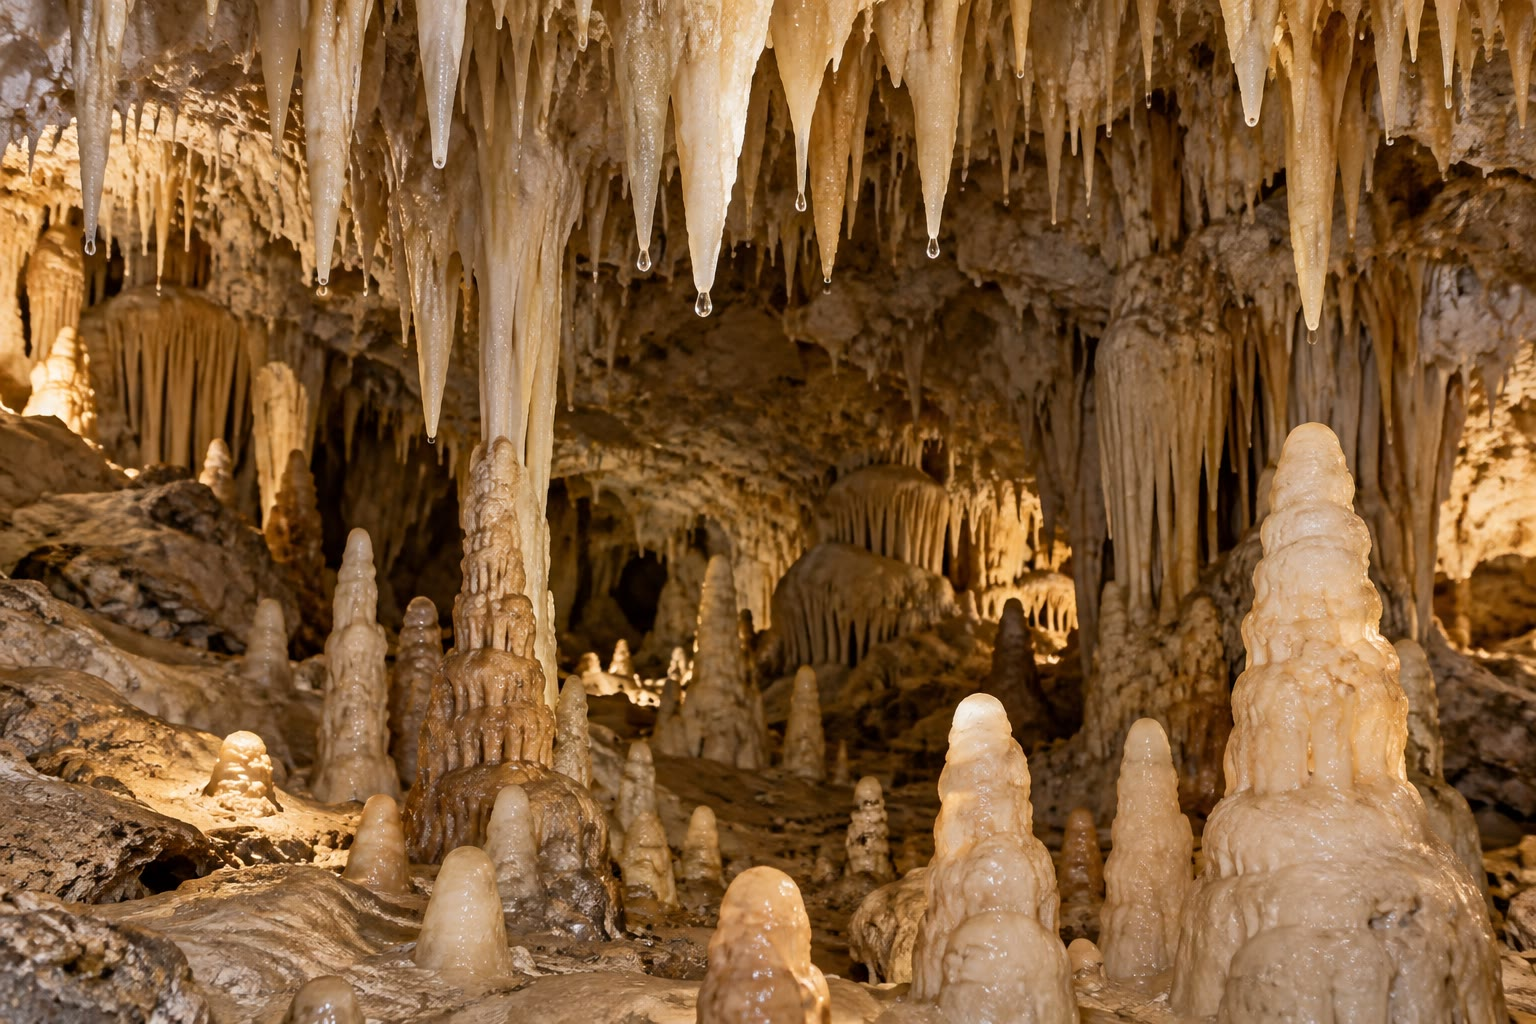
\includegraphics[width=0.45\linewidth]{images/book1/ai/g12-cave-stalactites.jpg}

{\small تنمو الهوابط حيث يفقد الماء المتقاطر في كهف ثنائي أكسيد
الكربون لصالح \omterm{def:g4:air-a-mixture-of-gases:air}{الهواء}: فينزاح توازن الحجر الجيري \omterm{def:g6:solutions-and-solubility:solute}{المذاب}،
وتترسب كربونات الكالسيوم.}
\end{omfigure}

\section{تمارين}

\begin{exercise}[$\star$]\label{exo:g12:equilibrium:1}
اكتب \omterm{def:g12:equilibrium:quotient}{خارج التفاعل} لكل من: (a) \ce{N2 + 3H2 <=> 2NH3} (غازات، استعمل
التراكيز)؛ (b) \ce{CH3COOH + H2O <=> CH3COO- + H3O+} في الماء؛
(c) \ce{CaCO3(s) <=> Ca^{2+} + CO3^{2-}}؛ (d) \ce{Fe^{3+} + SCN- <=>
FeSCN^{2+}}.
\end{exercise}

\begin{exercise}[$\star$]\label{exo:g12:equilibrium:2}
لتفاعل $x_{\max} = \qty{0.050}{mol}$، وهو يبلغ
$x_f = \qty{0.020}{mol}$. احسب $\tau$. أهو \omterm{def:g10:reaction-progress-table:limiting}{تفاعل تام}؟
\end{exercise}

\begin{exercise}[$\star$]\label{exo:g12:equilibrium:3}
لتفاعل ثابت توازنه $K = 10$، في أي اتجاه يتطور \omterm{def:g6:pure-substances-and-mixtures:mixture}{خليط} إذا كان
$Q = 2$؟ وإذا كان $Q = 50$؟ وإذا كان $Q = 10$؟
\end{exercise}

\begin{exercise}[$\star$]\label{exo:g12:equilibrium:4}
اشرح لماذا يُقال إن التوازن «ديناميكي».
\end{exercise}

\begin{exercise}[$\star$]\label{exo:g12:equilibrium:5}
أيغيّر \omterm{def:g12:catalysis:catalyst}{الحفّاز} $K$؟ وهل يغيّر المدة اللازمة لبلوغ التوازن؟ اشرح.
\end{exercise}

\begin{exercise}[$\star\star$]\label{exo:g12:equilibrium:6}
يُخلط \qty{2.0}{mol} من حمض الإيثانويك و\qty{2.0}{mol} من الإيثانول
($K = 4$). احسب الكميات النهائية للأنواع الأربعة.
\end{exercise}

\begin{exercise}[$\star\star$]\label{exo:g12:equilibrium:7}
يحوي \omterm{def:g6:pure-substances-and-mixtures:mixture}{خليط} \qty{0.5}{mol} من كل من حمض الإيثانويك والإيثانول وإيثانوات
الإيثيل والماء. احسب $Q$. وفي أي اتجاه يتطور؟
\end{exercise}

\begin{exercise}[$\star\star$]\label{exo:g12:equilibrium:8}
مستعينًا بشكل التجربتين، اقرأ كمية \omterm{def:g11:functional-groups:carboxylic-acid}{الإستر} بعد
\qty{20}{h} في كل تجربة. ومتى يمكن اعتبار المجموعة في
\omterm{def:g12:equilibrium:equilibrium-state}{حالة توازن}؟
\end{exercise}

\begin{exercise}[$\star\star$]\label{exo:g12:equilibrium:9}
انطلاقًا من \qty{1}{mol} من \omterm{def:g11:functional-groups:carboxylic-acid}{الإستر} و\qty{1}{mol} من الماء ($K = 4$
للأسترة، إذن $1/4$ للحلمأة)، احسب الكميات النهائية
بطريقة الفصل، وقارن بتجربة
الأسترة.
\end{exercise}

\begin{exercise}[$\star\star$]\label{exo:g12:equilibrium:10}
لماذا لا يظهر الجسم الصلب في \omterm{def:g12:equilibrium:quotient}{خارج التفاعل}
\ce{AgCl(s) <=> Ag+ + Cl-}؟ وهل تزيح إضافة مزيد من الصلب
التوازن؟
\end{exercise}

\begin{exercise}[$\star\star$]\label{exo:g12:equilibrium:11}
في قارورة ماء فوّار مغلقة، يغادر ثنائي أكسيد الكربون الماء ويدخله
بالسرعة نفسها. اكتب التوازن
\ce{CO2(aq) <=> CO2(g)} واشرح، مستعينًا \omterm{def:g12:equilibrium:quotient}{بخارج التفاعل} $Q$ وبالثابت $K$، لماذا يفقد الماء فورانه
حين تُفتح القارورة.
\end{exercise}

\begin{exercise}[$\star\star\star$]\label{exo:g12:equilibrium:12}
تبلغ أسترة \qty{1}{mol} من الحمض و\qty{1}{mol} من \omterm{def:g11:functional-groups:alcohol}{الكحول}
التوازن. ثم يُنزع نصف الماء الموجود. احسب
\omterm{def:g12:equilibrium:quotient}{خارج التفاعل} $Q$ الجديد، وقل في أي اتجاه تتطور المجموعة، وجد كمية \omterm{def:g11:functional-groups:carboxylic-acid}{الإستر}
النهائية الجديدة.
\end{exercise}

\begin{exercise}[$\star\star\star$]\label{exo:g12:equilibrium:13}
بيّن أن ثابت التفاعل العكسي هو $1/K$. وما
ثابت حلمأة إيثانوات الإيثيل؟
\end{exercise}

\begin{exercise}[$\star\star\star$]\label{exo:g12:equilibrium:14}
يخلط كيميائي \qty{1}{mol} من الحمض، و\qty{1}{mol} من \omterm{def:g11:functional-groups:alcohol}{الكحول}،
و\qty{2}{mol} من \omterm{def:g11:functional-groups:carboxylic-acid}{الإستر} و\qty{0.5}{mol} من الماء. أسيحدث شيء؟
اشرح.
\end{exercise}

\begin{exercise}[$\star\star\star$]\label{exo:g12:equilibrium:15}
ما فائض \omterm{def:g11:functional-groups:alcohol}{الكحول} (الكمية لكل \omterm{def:g10:the-mole:amount}{مول} من الحمض) اللازم لأسترة
\qty{95}{\percent} من الحمض؟ حلّ $\dfrac{0.95^2}{0.05(n - 0.95)} =
4$.
\end{exercise}

\section{مسألة: إستر برتلو}

\begin{problem}[{مسألة نهاية الأسبوع --- كم من الإستر حين يوضع الكحول
بفائض ثلاثة أضعاف؟}]
\label{pb:g12:equilibrium:1}
% ledger: ester:berthelot, aw:C, aw:H, aw:O
إيثانوات الإيثيل، وهي \omterm{def:g6:solutions-and-solubility:solute}{مذيب} ومنكّه، تُحضَّر من حمض الإيثانويك
والإيثانول. وفي سنة 1862 وجد برتلو وبيان دو سان-جيل أنه انطلاقًا من
كميتين متساويتين من الحمض \omterm{def:g11:functional-groups:alcohol}{والكحول} يتوقف التفاعل حين يكون نحو الثلثين
من الحمض قد تفاعلا.

\medskip
\noindent\textbf{الجزء الأول --- التفاعل.}
\begin{enumerate}
  \item اكتب معادلة الأسترة، بالصيغ نصف
        البنيوية.
  \item لماذا تُكتب بسهم مزدوج؟
  \item اكتب خارج تفاعلها بدلالة الكميات.
  \item انطلاقًا من \qty{1}{mol} من الحمض و\qty{1}{mol} من \omterm{def:g11:functional-groups:alcohol}{الكحول}، ما
        $x_{\max}$؟ وما $x_f$ بحسب نتيجة برتلو؟
  \item احسب $\tau$.
\end{enumerate}

\medskip
\noindent\textbf{الجزء الثاني --- الثابت.}
\begin{enumerate}[resume]
  \item أعطِ الكميات النهائية للأنواع الأربعة.
  \item احسب $K$.
  \item انطلاقًا من \qty{1}{mol} من \omterm{def:g11:functional-groups:carboxylic-acid}{الإستر} و\qty{1}{mol} من الماء،
        وجد برتلو أن الثلث قد تحلمأ. بيّن أن هذا يتفق مع
        قيمة $K$ نفسها.
  \item لماذا يجب أن يكون $K$ هو نفسه في الحالتين؟
\end{enumerate}

\medskip
\noindent\textbf{الجزء الثالث --- فائض من \omterm{def:g11:functional-groups:alcohol}{الكحول} بثلاثة أضعاف.}
\begin{enumerate}[resume]
  \item انطلاقًا من \qty{1}{mol} من الحمض و\qty{3}{mol} من \omterm{def:g11:functional-groups:alcohol}{الكحول}، املأ
        \omterm{def:g10:reaction-progress-table:extent}{جدول التقدم}.
  \item اكتب المعادلة $Q_{eq} = K$ وبيّن أنها تصير
        $3x^2 - 16x + 12 = 0$.
  \item حلّها، واحتفظ بالجذر ذي المعنى.
  \item ما الكسر المستَر من الحمض؟
  \item احسب كتلة \omterm{def:g11:functional-groups:carboxylic-acid}{الإستر} المحصّلة.
\end{enumerate}

\medskip
\noindent\textbf{الجزء الرابع --- نزع الماء.}
\begin{enumerate}[resume]
  \item انطلاقًا من التوازن المتساوي المولات، يُنزع الماء حالما
        يتكوّن. اشرح بواسطة $Q$ لماذا يستمر التفاعل.
  \item لو أمكن نزع الماء كله، فكم يصير \omterm{def:g10:synthesis-yield:yield}{المردود}؟
  \item لماذا يوضع \omterm{def:g11:functional-groups:alcohol}{الكحول}، لا الحمض، بفائض في العادة؟ (فكّر
        في الكلفة وفي فصل \omterm{def:g7:chemical-reactions:reactant}{النواتج}.)
  \item أيغيّر تسخين \omterm{def:g6:pure-substances-and-mixtures:mixture}{الخليط} \omterm{def:g10:reaction-progress-table:system}{الحالة النهائية}، أم المدة اللازمة
        لبلوغها فقط؟ (فالأسترة لا تكاد تطلق حرارة.)
  \item اذكر الجواب النهائي: ما الكسر المستَر من الحمض
        مع فائض من \omterm{def:g11:functional-groups:alcohol}{الكحول} بثلاثة أضعاف؟
\end{enumerate}
\end{problem}
